\newcommand{\posterSummary}[1]{

\setlength{\frameWidth}{#1}
\setlength{\unitlength}{0.02\frameWidth}
\psset{unit=\unitlength}


\rput[t](44,30){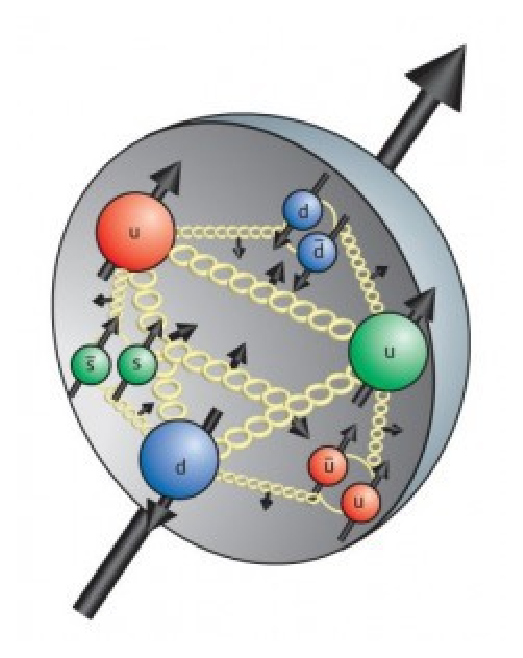
\includegraphics[width=11\unitlength]{graphics/proton}}

\rput[lt](2,29.5) {%
\begin{minipage}{40\unitlength}
\raggedright
\begin{list}{\labelitemi}{\setlength{\itemsep}{1mm}
                          \setlength{\topsep}{0mm}
                          \setlength{\leftmargin}{0mm}
                          \setlength{\rightmargin}{0mm} }

   \item \textbf{RHIC polarimeters are unique scientific tools at BNL}

   \begin{list}{\labelitemii}{\setlength{\topsep}{0mm}\setlength{\itemsep}{3mm}}
      \item Perform undestructive measurement of proton beam polarization
      \item Provide polarization measurements for all spin analyses at RHIC
      \item Provide valuable feedback to the RHIC machine operators
   \end{list}

\end{list}
\end{minipage}
}

\rput[lt](1,14){
\includegraphics[width=11\unitlength]{graphics/nanotube}}

\rput[lt](10,14) {%
\begin{minipage}{42\unitlength}
\raggedright
\begin{list}{\labelitemi}{\setlength{\itemsep}{1mm}
                          \setlength{\topsep}{0mm}
                          \setlength{\leftmargin}{0mm}
                          \setlength{\rightmargin}{0mm} }
   \item {\bf Future plans:}

   \begin{list}{\labelitemii}{\setlength{\itemsep}{1mm}}

      \item Next RHIC Run in 2013 we expect more data and $\sim +5$\% in polarization
      \item Ongoing studies aim to improve systematic uncertainties

      \begin{list}{\labelitemiii}{\setlength{\topsep}{1mm}\setlength{\itemsep}{1mm}}
         \item Different geometry and production techniques for carbon targets
         \item Cleaner signal selection in recoil samples
      \end{list}

   \end{list}

\end{list}
\end{minipage}
}


%\rput{0}{\psgrid[gridlabels=0.7,subgriddiv=0, griddots=3](1,-1)(0,0)(\myPsPictureWidthLocal,\myPsPictureHeightLocal)}

}

\setlength{\unitlength}{10mm}
\psset{unit=\unitlength}
